\pdfoutput=1
% arXiv submission: compile with pdfLaTeX (latexmk -pdf main).
\documentclass{article}

\usepackage{arxiv}% template: github.com/kourgeorge/arxiv-style
\raggedbottom
\usepackage[utf8]{inputenc}
\usepackage[T1]{fontenc}
\usepackage{textcomp}
\usepackage{amsmath,amssymb,amsthm,mathtools,bm}
\usepackage{booktabs,threeparttable,tabularx,makecell,multirow,array}
\usepackage{graphicx,float}
\usepackage[font=small,labelfont=bf,labelsep=period,justification=justified,singlelinecheck=false,skip=6pt]{caption}
\usepackage{xcolor}
\usepackage{tikz}
\usetikzlibrary{arrows.meta,positioning,fit,calc,backgrounds,shapes.geometric}
\usepackage{enumitem}
\usepackage{microtype}
\usepackage[authoryear,round]{natbib}
\usepackage[most]{tcolorbox}
\usepackage{url}

\definecolor{ink}{HTML}{1D2330}
\definecolor{muted}{HTML}{6B7280}
\definecolor{faint}{HTML}{9CA3AF}
\definecolor{rule}{HTML}{E6E8EC}
\definecolor{thai}{HTML}{B5172B}
\definecolor{tron}{HTML}{E4572E}
\definecolor{ethblue}{HTML}{3D5A80}
\definecolor{teal}{HTML}{2A9D8F}
\definecolor{amber}{HTML}{E09F3E}
\definecolor{legit}{HTML}{94A3B8}

\usepackage[colorlinks=true,linkcolor=thai,citecolor=ethblue,urlcolor=teal,
  pdftitle={Shadow Dollars: Stablecoin Rails, Scam Finance and the Limits of Detection in Thailand},
  pdfauthor={Thanatchon Chongmankhong},
  pdfkeywords={stablecoins, USDT, Tron, money laundering, scam centres, bunching, synthetic control, Thailand}]{hyperref}
\usepackage[capitalise,noabbrev]{cleveref}

\renewcommand{\topfraction}{0.92}
\renewcommand{\bottomfraction}{0.6}
\renewcommand{\textfraction}{0.06}
\renewcommand{\floatpagefraction}{0.85}
\setcounter{topnumber}{3}
\setcounter{bottomnumber}{2}
\setcounter{totalnumber}{5}
\setcounter{tocdepth}{1}
\setlength{\emergencystretch}{1.5em}
\makeatletter
% float pages: stack floats from the top instead of centring them vertically
\setlength{\@fptop}{0pt}
\setlength{\@fpsep}{14pt plus 4pt}
\setlength{\@fpbot}{0pt plus 1fil}
\makeatother
% the template forbids every widow and club line; allow them at a cost so pages fill
\widowpenalty=1500
\clubpenalty=1500

\theoremstyle{plain}
\newtheorem{proposition}{Proposition}
\newtheorem{corollary}{Corollary}
\newtheorem{lemma}{Lemma}
\theoremstyle{definition}
\newtheorem{assumption}{Assumption}
\renewcommand{\theassumption}{A\arabic{assumption}}
\newtheorem{definition}{Definition}
\theoremstyle{remark}
\newtheorem{remark}{Remark}

\newcommand{\fig}[2]{\includegraphics[width=#1\textwidth]{figures/#2.pdf}}
\newcommand{\E}{\mathbb{E}}
\newcommand{\1}{\mathbf{1}}
\newcolumntype{L}[1]{>{\raggedright\arraybackslash}p{#1}}
\setlist{itemsep=0.15em,topsep=0.35em}
\crefname{assumption}{Assumption}{Assumptions}
\crefname{proposition}{Proposition}{Propositions}

\tcbset{findings/.style={enhanced,breakable,colback=white,colframe=thai,boxrule=0pt,
  leftrule=2.2pt,arc=0pt,outer arc=0pt,left=10pt,right=8pt,top=6pt,bottom=6pt,
  fonttitle=\bfseries\color{thai},coltitle=thai,colbacktitle=white,
  title style={fill=white},attach title to upper,after title={\par\smallskip}}}

% ------------------------------------------------------------- arXiv template fields
\renewcommand{\headeright}{A Preprint}
\renewcommand{\undertitle}{A Preprint}
\renewcommand{\shorttitle}{Shadow Dollars}

\title{Shadow Dollars: Stablecoin Rails, Scam Finance and the Limits of Detection in Thailand}

\author{Thanatchon Chongmankhong}
% Optional: add affiliation and e-mail on new lines inside \author{...}, e.g.
% \author{Thanatchon Chongmankhong\\ Affiliation\\ \texttt{email@example.com}}

\date{November 8, 2026}

\begin{document}
\maketitle

\begin{abstract}
Thailand combines low inflation, a licensed and identity-verified crypto exchange sector, and a long border with the
scam-compound economy of Myanmar, Cambodia and Laos. I ask whether Thai stablecoin behaviour is anomalous, whether
USDT is a plausible channel for laundering transnational fraud proceeds, and how either claim can be tested credibly.
Public on-chain data through May 2026 show that USDT on Tron is a retail dollar rail distinct from USDT on Ethereum: it
carries 47\% of the covered USDT supply, 74.5 million funded addresses (5.3 times Ethereum), mean balances about six
times smaller and 9.3 times the transfer intensity per dollar. Ninety-five per cent of U.S.\ sanctions-list addresses
tagged USDT, TRX or USDC are Tron addresses. Thailand itself has little macroeconomic reason to hold dollars on-chain
(2019--2023 inflation of 1.7\% a year, fourth lowest of 23 comparators), unlike neighbouring Laos and Myanmar.
Chain-wide data cannot evaluate national enforcement: nominal 95\% bands reject at 58\% of 149 placebo dates, and
placebo-calibrated p-values for three crackdowns range from 0.69 to 1.00. I therefore develop a pre-registered design
with four estimators---a difference-in-bunching test at the 50,000-baht face-verification threshold, dwell-time
mixtures, direction-aware graph exposure and synthetic control---and validate them in an agent-based simulation with
planted mule accounts. The common undirected two-hop exposure rule attains 2--6\% precision among top-ranked accounts;
multi-signal scoring reaches 78--92\%; the bunching-difference test has close-to-nominal size and 88\% power at a 2\%
mule share. A channel-choice model explains why enforcement that displaces flows leaves chain-wide totals unchanged.
Code and data are released for replication.
\end{abstract}

\keywords{stablecoins \and USDT \and Tron \and money laundering \and scam centres \and bunching \and synthetic control
\and blockchain forensics \and Thailand}

\smallskip
\noindent{\bfseries\emph{JEL codes}}\enspace E42, G23, G28, K42, C63, O53

\vspace{1.2em}
\begin{tcolorbox}[findings,title={Key findings},fontupper=\small]
\begin{enumerate}[leftmargin=1.4em,label=\textbf{\arabic*.},itemsep=0.05em,topsep=0.1em]
\item \textbf{A distinct rail.} USDT on Tron is a high-turnover, small-balance dollar rail: 47\% of covered USDT supply,
74.5 million funded addresses and 9.3 times the transfer intensity of USDT on Ethereum (\cref{sec:rails}).
\item \textbf{A weak macro motive.} Thai inflation and exchange-rate volatility do not explain heavy stablecoin use; the
same is not true of neighbouring Laos and Myanmar, whose legitimate dollar demand can flow through Thai channels (\cref{sec:macro}).
\item \textbf{Aggregate data mislead.} Chain-level event studies over-reject at 58\% of random dates; with honest,
placebo-calibrated inference no crackdown is detectable, which a displacement model predicts (\cref{sec:eventstudy,sec:displacement}).
\item \textbf{Detect differences, follow direction.} Structuring is identified by the \emph{difference} in bunching
between USDT and other assets, not by bunching itself; graph exposure must follow the direction of funds (\cref{sec:sim}).
\item \textbf{A ready design.} Six pre-registered hypotheses, decision rules and open code make the Thai question
testable as soon as exchange or regulator data are available under the PDPA (\cref{sec:plan}).
\end{enumerate}
\end{tcolorbox}

\newpage
\section{Introduction}\label{sec:intro}

Stablecoins have become the settlement asset of the crypto economy and, increasingly, a dollar substitute for people
outside the United States. They have also become the preferred medium of the industrialised online fraud that grew
out of Southeast Asia's border casinos and special economic zones. Regional and international bodies describe a
system in which victims' bank transfers are converted, through networks of rented accounts, into USDT on the Tron
blockchain and moved through informal ``guarantee'' marketplaces and underground bankers before being integrated into
real assets \citep{unodc2024casinos,unodc2025inflection,fatf2023cyberfraud}. Thailand sits at the edge of this system.
It hosts a licensed, identity-verified crypto exchange industry and a large retail investor base; it shares long land
borders with the compounds of Myawaddy, the casinos of Poipet and the special economic zones of the Golden Triangle;
and its banks, police and regulators have spent the past four years tightening controls on so-called mule accounts.

This paper asks three questions that a Thai regulator, an exchange compliance officer or a researcher would want
answered. First, is Thai stablecoin behaviour unusual---relative to other crypto-assets traded on the same platforms
and relative to stablecoin use elsewhere? Second, is it plausible that criminal networks, including the ``call
centre'' fraud gangs that target Thai victims, launder proceeds through USDT, and through Thai rails in particular?
Third, and most important, how could either claim be tested in a way that separates criminal flows from the many
legitimate reasons to hold and move digital dollars?

The third question disciplines the first two. Unusual behaviour is not evidence of crime. Thai investors cannot trade
crypto derivatives on licensed domestic venues, so buying USDT and withdrawing it to an offshore exchange is the
ordinary route to leverage. Millions of migrant workers from Myanmar, Cambodia and Laos live in Thailand and send money
home, and two of those countries have recently experienced the high inflation and capital controls that make dollar
stablecoins attractive. Honest peer-to-peer dealers receive baht from many counterparties and withdraw quickly, which
is exactly what a mule account does. A credible study must therefore name each legitimate motive, state the
fingerprint it leaves in data, and show that the residual pattern attributed to laundering survives once those
fingerprints are removed.

\paragraph{What this paper does}
I make four contributions. The first is \emph{descriptive and uses only public data}. Using the Coin Metrics community
files through 23 May 2026, I document that USDT on Tron behaves as a retail payment rail that is economically distinct
from USDT on Ethereum (\cref{sec:rails}). Tron carries 47\% of the USDT supply on the chains covered by the data, up
from 19\% at the end of 2019. It hosts 74.5 million addresses with a positive balance---5.3 times as many as USDT on
Ethereum---with a mean balance of about US\$1,200 against roughly US\$7,000, and it records 9.3 times as many transfers
per dollar of supply. When Circle wound down USDC on Tron in 2024, USDC supply there fell from a peak of US\$3.5
billion to under US\$30 million, leaving the cheapest high-liquidity dollar rail in the region to a single issuer. In
the U.S.\ Treasury's sanctions list, 95\% of the addresses tagged USDT, TRX or USDC are Tron addresses. I also show that
Thailand's macroeconomic fundamentals give its residents little reason to hold dollars on-chain---its consumer-price
inflation averaged 1.7\% a year over 2019--2023, the fourth lowest of 23 comparators---whereas Laos (14.9\%) and Myanmar
have strong legitimate demand (\cref{sec:macro}).

The second contribution is \emph{a negative result with a methodological lesson}. Event studies on chain-wide activity
are a tempting way to evaluate crackdowns because the data are free. I estimate abnormal Tron USDT activity around
three dated shocks---Thailand's February 2025 power cut to border scam hubs, its June 2025 block on unlicensed offshore
exchanges, and the October 2025 U.S.\ and U.K.\ sanctions on Prince Group---and calibrate inference against 149 placebo
dates. Conventional bootstrap bands, which already account for serial correlation and trend uncertainty, reject the
null at 58\% of random dates. Calibrated against the placebo distribution, none of the three shocks is distinguishable
from an ordinary week ($p$ between 0.69 and 1.00). \Cref{sec:displacement} rationalises this: in a channel-choice model
in which enforcement raises the cost of one rail, flows are displaced to substitutes and the aggregate is unchanged to
first order.

The third contribution is \emph{a set of estimators matched to the economics of structuring and pass-through}
(\cref{sec:framework}). The central one exploits the Bank of Thailand's face-verification rule, which applies to
transfers of 50,000 baht or more. Honest users also dislike the scan and bunch below the threshold, so bunching by
itself proves nothing. Under an assumption that hassle avoidance is the same across the assets a deposit funds, the
\emph{difference} in a slope-invariant bunching statistic between USDT-funding and other deposits identifies the volume
of structured deposits (\cref{prop:bunching}). I complement it with dwell-time mixtures, a direction-aware measure of
graph exposure to flagged addresses, and synthetic control for policy shocks, and I prove that undirected hop counts
mechanically flag exchange hubs (\cref{prop:direction}).

The fourth contribution is \emph{validation}. Because no public dataset links Thai exchange accounts to criminal
outcomes, I build an agent-based simulator of an exchange-year with five honest populations (domestic traders,
offshore bridge traders including arbitrageurs, cross-border remitters, holders and honest peer-to-peer merchants) and
mule accounts whose tradecraft varies, including camouflaged mules on rented, aged accounts (\cref{sec:sim}). Against
planted ground truth, the undirected two-hop rule attains a precision of 2--6\% among its top-ranked accounts; speed
alone attains 6--21\%; a direction-aware exposure measure rises from 2\% to 86\% as prevalence grows; and multi-signal
scoring reaches 78--92\%. The bunching-difference test rejects in 7.5\% of null simulations at a nominal 5\% level and
in 88\% of simulations with 2\% mule accounts. Synthetic control has a 2.5\% false-rejection rate and 82\% power for a
0.10 log-point effect. These magnitudes are properties of the simulator; the ranking of methods and their failure modes
are the transferable result.

\paragraph{What this paper does not claim}
The paper does not estimate how much Thai stablecoin volume is criminal. Doing so requires account-level data that
exchanges and the Anti-Money Laundering Office hold and that the Personal Data Protection Act rightly restricts.
Instead, \cref{sec:plan} sets out a pre-registered plan---six hypotheses, the data tier each needs, the estimator and
the decision rule---so that the question can be answered as soon as such data are available, without specification
search. All code is open, every figure is regenerated from raw files whose checksums are recorded, and every
simulated figure is marked as such.

\paragraph{Roadmap}
\Cref{sec:background} describes the Thai regime and the regional scam economy. \Cref{sec:literature} relates the paper
to work on stablecoins, illicit crypto finance and blockchain forensics. \Cref{sec:framework} presents the conceptual
framework, the model and the propositions. \Cref{sec:data} describes the data. \Cref{sec:evidence} reports the
evidence from public data and \cref{sec:sim} the simulation study. \Cref{sec:plan} contains the pre-registered plan,
policy implications, limitations and conclusions. Proofs, simulator parameters and replication instructions are in the
appendix.

\section{Institutional background}\label{sec:background}

This section summarises the rules that shape how stablecoins can be used in Thailand and the regional criminal economy
that motivates the paper.\footnote{Institutional details and dates in this section were compiled from public announcements and are stated at the precision available, often the month. They should be checked against primary legal sources before being relied upon.}

\subsection{Thailand's digital-asset regime}

Crypto exchanges, brokers and dealers serving Thai residents must be licensed by the Securities and Exchange
Commission under the Emergency Decree on Digital Asset Businesses of 2018. The licensed market has long been
concentrated, with Bitkub holding a dominant share, and it was joined in early 2024 by a joint venture between Gulf
Energy and Binance. Five features of the regime matter for stablecoin behaviour.

\begin{enumerate}[leftmargin=1.4em,label=(\roman*)]
\item \emph{Baht-quoted trading.} Licensed venues have historically quoted assets against the baht; USDT and USDC were
added to the list of crypto-assets that may serve as quote assets only in early 2025. Before then the USDT/THB pair was
the main gate between baht and on-chain dollars.
\item \emph{No domestic derivatives.} Licensed exchanges do not offer leveraged crypto derivatives. Residents who want
leverage buy USDT at home and withdraw it to an offshore venue, which mechanically raises the withdrawal rate of USDT
relative to other assets.
\item \emph{No payments.} Since 2022 licensed businesses may not facilitate the use of crypto-assets to pay for goods and
services, so payment use, where it exists, migrates to peer-to-peer and over-the-counter channels that are harder to
observe.
\item \emph{Tax.} In 2025 the government approved a five-year exemption from personal income tax on gains from sales
through licensed Thai providers (2025--2029), raising the return to trading onshore.
\item \emph{Access to offshore venues.} In mid-2025 the authorities blocked access to several unlicensed foreign
exchanges, a shock that should displace some activity towards peer-to-peer markets and virtual private networks.
\end{enumerate}

\subsection{The anti-fraud architecture}

Thailand's response to online fraud has concentrated on the bank accounts through which victims' money first moves.
The Emergency Decree on Measures for the Prevention and Suppression of Technology Crimes of 2023 made it an offence to
open, rent out or sell accounts for others to use, and it allowed financial institutions to suspend suspicious
transfers and share information. An amendment in 2025 extended these duties to digital-asset business operators and
introduced liability for institutions whose negligence enables losses. The police established the Anti Online Scam
Operation Center, reachable through the 1441 hotline, in late 2023. Since 2023 banks have also required facial
biometric verification for transfers of roughly 50,000 baht or more per transaction, or 200,000 baht or more per day,
and for raising transfer limits.

These measures raise the cost of the classic chain in which a victim's transfer passes through several layers of mule
bank accounts before being withdrawn in cash. They create two predictions that this paper turns into tests. The
verification threshold should generate structuring---deposits placed just below 50,000 baht---in the channel that
launderers use (\cref{sec:bunching}). And tighter bank-side controls should displace laundering towards channels in
which baht leave the banking system quickly, of which converting them into USDT is the most liquid (\cref{sec:displacement}).

\subsection{The regional scam economy}

UNODC's 2024 report on casinos, underground banking and transnational organised crime in East and Southeast Asia
describes how criminal groups that grew out of junket and casino operations moved into large-scale online fraud run
from compounds in Myanmar, Cambodia and Laos, staffed in part by trafficked workers, and how they settle and launder
proceeds through underground banking and stablecoins, with USDT on Tron prominent among them \citep{unodc2024casinos}.
A 2025 follow-up documents the industry's spread to other regions \citep{unodc2025inflection}. The FATF's report on
cyber-enabled fraud describes the same pipeline from the perspective of financial intelligence units
\citep{fatf2023cyberfraud}, and its 2025 update on virtual assets highlights the growing use of stablecoins by illicit
actors \citep{fatf2025targeted}. Industry analysts report that stablecoins account for a majority of the transaction
volume received by addresses they classify as illicit \citep{chainalysis2025crime}.

Enforcement against this infrastructure intensified in 2024 and 2025. Tether, the Tron Foundation and TRM Labs formed a
financial crime unit to freeze USDT linked to crime. Research by blockchain analytics firms exposed Telegram-based
``guarantee'' marketplaces associated with the Cambodian conglomerate Huione Group, several of which Telegram removed in
2025 \citep{elliptic2024huione}. In February 2025 Thailand cut electricity, internet and fuel supplies to areas across
the Myanmar border that host scam compounds. In October 2025 the U.S.\ and U.K.\ governments sanctioned the Cambodian
Prince Group and associated individuals and entities, the U.S.\ Department of Justice filed a forfeiture complaint
against roughly 127,000 bitcoin, and FinCEN acted to sever Huione Group from the U.S.\ financial system
\citep{ustreasury2025prince,fincen2025huione}. In the same month Myanmar's military raided the KK Park compound.

\Cref{fig:timeline} places these events on one time axis. Its message for empirical work is simple: nine of the
sixteen events fall in the nine months between February and October 2025. Any design that attributes a change in
Thai stablecoin flows to one of them must contend with the others, which is why the pre-registered plan relies on
narrow windows, control assets and placebo inference.

\begin{figure}[!htbp]
\centering
\fig{0.98}{fig_timeline}
\caption{Policy, enforcement and market events relevant to Thai stablecoin flows, 2022--2025. Dots on the left axis
sit at the true date; labels on the right are in chronological order. Colours mark the type of event. Month-level
dates are shown without a day and should be verified against primary sources.}
\label{fig:timeline}
\end{figure}

\section{Related literature}\label{sec:literature}

The paper connects four literatures.

\paragraph{The economics of stablecoins}
A first strand studies what keeps stablecoins at par and what they do to the rest of the financial system.
\citet{lyons2023stable} show how arbitrage capacity and the issuer's balance sheet determine deviations from the peg;
\citet{gorton2023wildcat} draw the analogy with free-banking-era private money; \citet{arner2020stablecoins} and the
\citet{bis2025aer} discuss risks and regulation, and \citet{liao2022stablecoins} the implications for bank funding.
Work on the interaction between stablecoin issuance and crypto prices includes \citet{griffin2020tether},
\citet{ante2021issuance} and \citet{kristoufek2021tethered}. This literature treats stablecoins mostly as a single
asset. I show that the same token on different blockchains serves different clienteles---USDT on Tron is a small-balance,
high-turnover rail, USDT on Ethereum a large-balance one---which matters for any analysis of who uses stablecoins and why.

\paragraph{Illicit finance in crypto-assets}
\citet{foley2019sex} estimate the share of bitcoin activity associated with illegal goods using network clustering.
\citet{cong2023anatomy} provide an anatomy of crypto-enabled cybercrime, and \citet{griffin2024slavery} trace the flows
of ``pig-butchering'' fraud from victims to exchanges, documenting the role of USDT and large centralised exchanges in
cashing out. Policy reports by \citet{unodc2024casinos,unodc2025inflection} and the
\citet{fatf2020redflags,fatf2023cyberfraud,fatf2025targeted} describe typologies and red flags. Industry reports such as
\citet{chainalysis2025crime} provide aggregate estimates whose attribution methods are proprietary. Relative to this
work I focus on a single jurisdiction at the boundary between the banking system and on-chain rails, and on the
identification problem: how to distinguish laundering from the legitimate motives that produce similar data.

\paragraph{Market structure and data quality}
\citet{makarov2020arbitrage} document persistent cross-country price premia in crypto markets, such as the Korean
``kimchi premium'', that reflect capital controls; I use the analogous USDT/THB premium as a fingerprint of the
store-of-value motive. \citet{cong2023wash} show that reported exchange volumes are inflated by wash trading, which is
why the plan relies on ratios within a platform and on adjusted volumes rather than on raw cross-exchange comparisons.
\citet{auer2022retail} relate retail adoption to prices using app-download data.

\paragraph{Blockchain forensics and anomaly detection}
Address clustering and labelling go back to \citet{meiklejohn2013fistful}; supervised and graph-based approaches to
anti-money-laundering on transaction graphs include \citet{weber2019aml}. I use unsupervised scores---the isolation forest
of \citet{liu2008iforest} and a transparent composite of red flags---because labels are scarce in practice, and I show
formally and in simulation that the direction of fund flows must be respected when exposure to flagged addresses is
measured. Community detection, used in the replication package for exploratory clustering, follows
\citet{blondel2008louvain}.

\paragraph{Methods}
The bunching estimator adapts the notch and kink designs of \citet{saez2010bunch}, \citet{chetty2011adjustment} and
\citet{kleven2013notches}, surveyed by \citet{kleven2016bunching}, to a setting in which the notch is a verification
step rather than a tax, and in which a within-platform comparison across assets removes the honest response. Policy
evaluation relies on synthetic control \citep{abadie2010synth,abadie2021using} and, as a robustness check, synthetic
difference-in-differences \citep{arkhangelsky2021sdid}. Cross-country controls include the capital-account openness
index of \citet{chinn2006capital}.

\section{Conceptual framework}\label{sec:framework}

\subsection{Four motives and their fingerprints}\label{sec:motives}

Observed stablecoin flows on Thai rails are the sum of four motives. \emph{Trading and offshore bridging}: residents buy
USDT as collateral or as the vehicle to reach offshore derivatives. \emph{Dollar saving}: residents hold USDT as a
store of value. \emph{Cross-border transfer}: migrant workers, traders and tourists move value across borders.
\emph{Illicit pass-through}: criminal proceeds enter as baht and leave as USDT. Each motive leaves a distinct
fingerprint, summarised in \cref{tab:motives}, and the identification strategy is to remove the first three before
interpreting the residual (\cref{fig:funnel}).

\begin{table}[!htbp]
\centering\small
\caption{Motives for holding and moving stablecoins on Thai rails, their fingerprints and how they are tested}
\label{tab:motives}
\begin{tabularx}{\textwidth}{L{2.6cm}XXc}
\toprule
Motive & Fingerprint in the data & Main confounder & Hypothesis \\
\midrule
Trading and offshore bridge & USDT volume co-moves with crypto volatility and offshore funding rates; withdrawals go
to labelled exchange hot wallets and return after gains & Arbitrageurs move as fast as mules & H1, H2 \\
\addlinespace
Dollar saving & Long holding periods; USDT/THB premium over the official rate rises when the baht weakens & Little
in Thailand (low inflation) & H1 \\
\addlinespace
Cross-border transfer & Small, regular amounts; peaks after paydays and before festivals; destinations are P2P desks in
neighbouring countries & Tainted P2P merchants & H1, H6 \\
\addlinespace
Illicit pass-through & Young accounts funded by many bank accounts; deposits structured below 50,000 baht; exits within
minutes; forward paths to flagged addresses; responds to crackdowns, not prices & Honest P2P dealers, camouflaged mules
& H3--H6 \\
\bottomrule
\end{tabularx}
\end{table}

\begin{figure}[!htbp]
\centering
\begin{tikzpicture}[
  font=\sffamily\scriptsize, >={Stealth[length=2.2mm]}, every node/.append style={execute at begin node={\hyphenpenalty=10000\exhyphenpenalty=10000}},
  stage/.style={draw=faint, line width=0.5pt, fill=rule!45, text width=2.5cm, align=center, inner sep=4pt},
  last/.style={draw=thai, line width=1pt, fill=thai!10, text width=2.5cm, align=center, inner sep=4pt},
  note/.style={text width=2.75cm, align=center, text=muted, font=\sffamily\tiny, inner sep=1pt},
  test/.style={text width=2.95cm, align=center, text=thai, font=\sffamily\tiny\bfseries, inner sep=1pt}]
\node[stage, minimum height=3.3cm] (a) at (0,0) {\textbf{All stablecoin flows on Thai rails}\\[3pt]exchange purchases, withdrawals,\\ P2P and OTC trades};
\node[stage, minimum height=2.7cm, right=0.55cm of a] (b) {\textbf{Net of trading and offshore bridging}};
\node[stage, minimum height=2.1cm, right=0.55cm of b] (c) {\textbf{Net of dollar saving}};
\node[stage, minimum height=1.6cm, right=0.55cm of c] (d) {\textbf{Net of cross-border transfers}};
\node[last, minimum height=1.1cm, right=0.55cm of d] (e) {\textbf{Residual to explain}};
\foreach \u/\v in {a/b,b/c,c/d,d/e} \draw[->, draw=muted, line width=0.6pt] (\u.east) -- (\v.west);
\node[note, below=0.25cm of a.south] (na) {observed volume, withdrawals, premium, network mix};
\node[note, anchor=north] at (na.north -| b) {control asset on the same platform; crypto volatility; exchange-labelled destinations};
\node[note, anchor=north] at (na.north -| c) {USDT/THB premium versus the reference rate; holding periods};
\node[note, anchor=north] at (na.north -| d) {payday and festival seasonality; destinations in neighbouring countries};
\node[note, anchor=north] at (na.north -| e) {structuring, pass-through speed, fan-in, forward exposure};
\node[test, above=0.2cm of a.north] (ta) {H1 excess demand};
\node[test, anchor=south] at (ta.south -| b) {H2 USDT vs.\ other assets};
\node[test, anchor=south] at (ta.south -| c) {H1 premium};
\node[test, anchor=south] at (ta.south -| d) {H1, H6 destinations};
\node[test, anchor=south] at (ta.south -| e) {H3 dwell \textperiodcentered{} H4 bunching\\H5 shocks \textperiodcentered{} H6 exposure};
\end{tikzpicture}
\caption{Identification strategy. Observed flows are the sum of four motives. Each legitimate motive is removed using
its fingerprint (grey notes) before the residual is interpreted; red labels give the pre-registered hypotheses of
\cref{sec:plan} that test each step. Box heights are schematic, not estimates.}
\label{fig:funnel}
\end{figure}

\subsection{Structuring at a verification notch}\label{sec:bunching}

Consider deposits of baht onto a licensed platform. Each deposit has an intended amount $z$ and funds an asset class
$a\in\{S,O\}$, where $S$ denotes USDT and $O$ any other crypto-asset. Banks require face verification for transfers of
at least $T$ baht. Let $h_a(z)$ be the counterfactual density of intended amounts of honest deposits funding $a$, and
write $H_a(A)=\int_A h_a(z)\,dz$ for the counterfactual mass in a set $A$.

Honest depositors whose intended amount lies in a response window $[T,T+R)$ relocate to a bunching window $[T-\delta,T)$
with probability $\pi_a(z)$; they find the scan a hassle, or simply prefer to split the transfer. Launderers add a mass
$I_a$ of \emph{structured} deposits placed in $[T-\delta,T)$ to avoid the verification step that would expose a mule's
identity. The observed excess mass below the threshold and the responding share are
\begin{equation}\label{eq:excess}
B_a=\int_T^{T+R}\pi_a(z)\,h_a(z)\,dz + I_a,
\qquad
\beta_a=\frac{B_a}{H_a\!\left([T,T+R)\right)}=\bar\pi_a+\frac{I_a}{H_a\!\left([T,T+R)\right)},
\end{equation}
where $\bar\pi_a$ is the average relocation probability over the response window.

\begin{assumption}[Asset-invariant hassle avoidance]\label{as:a1}
$\bar\pi_S=\bar\pi_O$: the share of honest deposits intended for the response window that relocate below $T$ does
not depend on which asset the deposit funds.
\end{assumption}
\begin{assumption}[Channel specificity]\label{as:a2}
$I_O=0$: structured deposits fund the stablecoin channel, which offers immediate, liquid exit.
\end{assumption}
\begin{assumption}[Smooth counterfactual]\label{as:a3}
$h_a$ is smooth in $\log z$ on a neighbourhood of $[T-\delta,T+R)$, so that it is identified from the observed density
outside that window, up to multiplicative round-number effects.
\end{assumption}

\begin{proposition}[Difference in bunching]\label{prop:bunching}
Under \cref{as:a1,as:a2,as:a3},
\[
\Delta\beta\equiv\beta_S-\beta_O=\frac{I_S}{H_S\!\left([T,T+R)\right)}\geq 0,
\]
with equality if and only if $I_S=0$. The structured stablecoin volume is identified as
$I_S=\Delta\beta\cdot H_S([T,T+R))$.
\end{proposition}

The proof is immediate from \cref{eq:excess} and is given in \cref{app:proofs}. Two features matter in practice. First,
the normalisation: the classic statistic divides the excess by the counterfactual density just below $T$. When the two
asset classes have amount distributions of different shapes---stablecoin deposits are larger---that statistic differs
across assets even when $\bar\pi_S=\bar\pi_O$. In the simulation below, a test based on it rejected a true null in 14\%
of draws at a nominal 5\% level; the responding share $\beta_a$ in \cref{eq:excess} reduced this to 7.5\%. Second,
\cref{as:a1} can be relaxed. If deposits observed before the verification rule exist, the change in $\Delta\beta$ across
the rule's introduction identifies $I_S$ under the weaker assumption that asset-specific differences in honest bunching
are stable over time.

\begin{corollary}[Difference-in-difference-in-bunching]\label{cor:didib}
If $\bar\pi_S-\bar\pi_O$ is the same before and after the rule's introduction and no structuring occurs at $T$ before
it, then $\Delta\beta^{\text{post}}-\Delta\beta^{\text{pre}}=I_S^{\text{post}}/H_S^{\text{post}}([T,T+R))$.
\end{corollary}

A placebo version of the test at amounts where no verification step exists ($T'$ = 30,000 or 70,000 baht) provides a
specification check: under correct specification $\Delta\beta(T')$ should be zero.

\subsection{Pass-through and the limits of speed}\label{sec:speed}

A mule account exists to move value, so the time between a baht deposit and the withdrawal of the USDT it bought---its
\emph{dwell time}---is short. But speed is shared with honest populations: arbitrageurs exploit price gaps within
minutes, and peer-to-peer dealers recycle inventory quickly. The following bound formalises why a speed-only rule
cannot achieve high precision when such populations exist.

\begin{lemma}[Speed is not sufficient]\label{lem:speed}
Let $n_M$ mule accounts and $n_F$ honest ``fast'' accounts have dwell times with distribution functions $G_M$ and
$G_F$, with $G_F(t)\geq G_M(t)$ for all $t$ (honest fast accounts are at least as fast). For any rule that flags
accounts with dwell time below a threshold $t$, the expected number of flagged mules divided by the expected number of
flagged accounts is at most $n_M/(n_M+n_F)$.
\end{lemma}

In the simulated economy of \cref{sec:sim} with 2\% mules, arbitrageurs and honest dealers make the bound about 0.25;
the speed-only score attains a precision of 0.12. Speed is a useful input to a score, not a test.

\subsection{Exposure to flagged addresses: direction matters}\label{sec:direction}

Compliance systems commonly flag an account if the destination of its withdrawals lies within $k$ hops of a sanctioned
or frozen address. Let $G=(V,E)$ be the directed graph of transfers, with edges pointing in the direction of funds, and
let $F\subset V$ be the flagged set. Let $d_u(v,F)$ be the undirected distance from $v$ to $F$ and $d_\to(v,F)$ the length
of the shortest \emph{forward} path from $v$ into $F$. For an account $i$ with withdrawals $w$ of value $x_w$ to
destinations $v_w$, define the value-weighted exposure
\begin{equation}\label{eq:exposure}
X_i^{(k)}=\frac{\sum_w x_w\,\1\{d(v_w,F)\leq k\}}{\sum_w x_w},\qquad d\in\{d_u,d_\to\}.
\end{equation}

\begin{proposition}[Hubs and undirected distance]\label{prop:direction}
Let $h$ be an exchange hot wallet that receives at least one payment from a wallet $\ell$ that pays a flagged address
($\ell\to f$, $f\in F$), and suppose every forward path from $h$ into $F$ has length at least $m>2$, or none exists. Then
$d_u(h,F)\leq 2$ while $d_\to(h,F)\geq m$. For $2\le k<m$, every account that withdraws only to $h$ has $X^{(k)}=1$
under undirected distance and $X^{(k)}=0$ under forward distance.
\end{proposition}

Large exchanges receive deposits from criminals cashing out, so in real data almost every exchange hot wallet satisfies
the premise. Because Thai residents who bridge to offshore venues withdraw to exactly these wallets, the undirected rule
generates false positives on the population that is largest and least suspicious. Forward distance removes this
artefact but not \emph{taint contagion}: an honest remitter who pays a peer-to-peer merchant that later pays a layering
wallet is exposed under both definitions, which motivates value weighting and the combination with behavioural signals.

\subsection{Displacement across channels}\label{sec:displacement}

Why might a crackdown leave no trace in chain-wide data? Suppose a laundering network must move a fixed volume $M$ of
proceeds through channels $j\in J$---for example licensed-exchange mule accounts ($E$), peer-to-peer desks ($P$) and
over-the-counter underground bankers ($U$)---with strictly convex costs $c_j(q_j)$. Enforcement raises the marginal
cost of channel $E$ by $\tau$. The network solves
\begin{equation}\label{eq:channels}
\min_{\{q_j\geq0\}}\ \sum_{j\in J}c_j(q_j)+\tau q_E\quad\text{subject to}\quad\sum_{j\in J}q_j=M .
\end{equation}

\begin{proposition}[Displacement]\label{prop:displacement}
At an interior optimum, $\partial q_E/\partial\tau=-(1-\omega_E)/c_E''<0$ and $\partial q_j/\partial\tau=\omega_E/c_j''>0$
for $j\neq E$, where $\omega_E=(1/c_E'')/\sum_{l\in J}(1/c_l'')\in(0,1)$. Total flow is unchanged:
$\sum_j\partial q_j/\partial\tau=0$.
\end{proposition}

\begin{corollary}[Invisible crackdowns]\label{cor:invisible}
If all channels terminate in the same on-chain asset, an enforcement shock that leaves $M$ unchanged has no first-order
effect on chain-level volume. If $M$ responds through deterrence, the effect on chain-level volume is bounded by the
network's share of that volume.
\end{corollary}

\Cref{cor:invisible} is the theoretical counterpart of the event-study result in \cref{sec:eventstudy}. It also says
where to look instead: the composition of flows---the share of fast, structured deposits on licensed platforms, the
peer-to-peer premium, the network mix---moves even when the total does not.

\subsection{Typology and control points}\label{sec:typology}

\Cref{fig:typology} summarises, at the level of generality used by the FATF and UNODC, the path of fraud proceeds and
the points at which Thai institutions can intervene. The conversion step is the boundary: before it, funds sit in the
domestic banking system where they can be frozen quickly; after it, they move on a public ledger where they can be
traced indefinitely and, for USDT, frozen by the issuer.

\begin{figure}[!htbp]
\centering
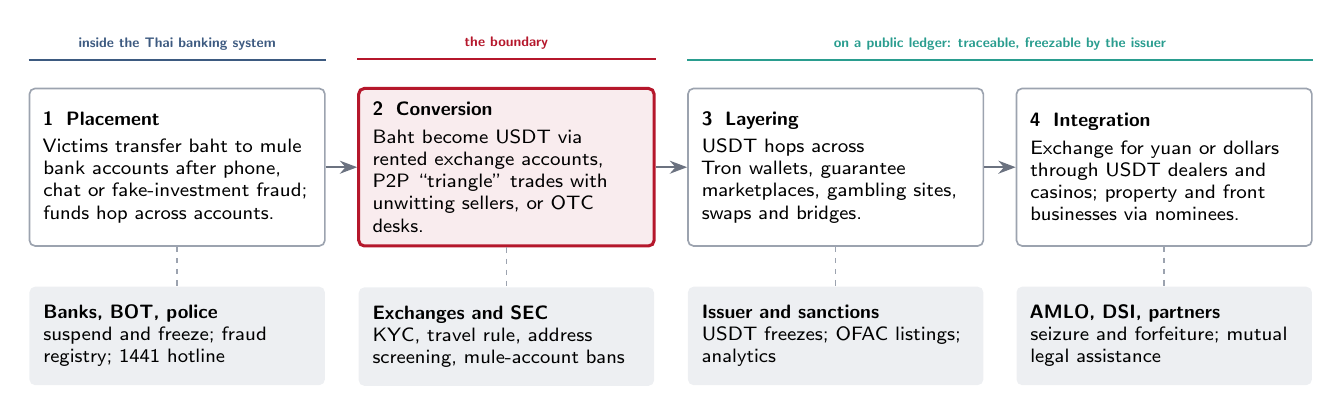
\begin{tikzpicture}[
  font=\sffamily\scriptsize, >={Stealth[length=2.2mm]}, every node/.append style={execute at begin node={\hyphenpenalty=10000\exhyphenpenalty=10000}},
  stg/.style={draw=faint, line width=0.6pt, rounded corners=2pt, text width=3.4cm, minimum height=2.0cm, align=left, inner sep=5pt, fill=white},
  key/.style={draw=thai, line width=1.1pt, rounded corners=2pt, text width=3.4cm, minimum height=2.0cm, align=left, inner sep=5pt, fill=thai!8},
  ctl/.style={rounded corners=2pt, text width=3.4cm, minimum height=1.25cm, align=left, inner sep=5pt, fill=rule!70}]
\node[stg] (s1) at (0,0) {\textbf{1\; Placement}\\[2pt]Victims transfer baht to mule bank accounts after phone, chat or fake-investment
fraud; funds hop across accounts.};
\node[key, right=0.4cm of s1] (s2) {\textbf{2\; Conversion}\\[2pt]Baht become USDT via rented exchange accounts, P2P ``triangle'' trades with
unwitting sellers, or OTC desks.};
\node[stg, right=0.4cm of s2] (s3) {\textbf{3\; Layering}\\[2pt]USDT hops across Tron wallets, guarantee marketplaces, gambling sites, swaps
and bridges.};
\node[stg, right=0.4cm of s3] (s4) {\textbf{4\; Integration}\\[2pt]Exchange for yuan or dollars through USDT dealers and casinos; property and
front businesses via nominees.};
\foreach \u/\v in {s1/s2,s2/s3,s3/s4} \draw[->, draw=muted, line width=0.7pt] (\u.east) -- (\v.west);
\node[ctl, below=0.5cm of s1] (c1) {\textbf{Banks, BOT, police}\\ suspend and freeze; fraud registry; 1441 hotline};
\node[ctl, below=0.5cm of s2] (c2) {\textbf{Exchanges and SEC}\\ KYC, travel rule, address screening, mule-account bans};
\node[ctl, below=0.5cm of s3] (c3) {\textbf{Issuer and sanctions}\\ USDT freezes; OFAC listings; analytics};
\node[ctl, below=0.5cm of s4] (c4) {\textbf{AMLO, DSI, partners}\\ seizure and forfeiture; mutual legal assistance};
\foreach \s/\c in {s1/c1,s2/c2,s3/c3,s4/c4} \draw[draw=faint, line width=0.6pt, dash pattern=on 2pt off 2pt] (\s.south) -- (\c.north);
\draw[line width=0.7pt, draw=ethblue] ([yshift=0.35cm]s1.north west) -- ([yshift=0.35cm]s1.north east)
  node[midway, above, text=ethblue, font=\sffamily\tiny\bfseries] {inside the Thai banking system};
\draw[line width=0.7pt, draw=teal] ([yshift=0.35cm]s3.north west) -- ([yshift=0.35cm]s4.north east)
  node[midway, above, text=teal, font=\sffamily\tiny\bfseries] {on a public ledger: traceable, freezable by the issuer};
\draw[line width=0.7pt, draw=thai] ([yshift=0.35cm]s2.north west) -- ([yshift=0.35cm]s2.north east)
  node[midway, above, text=thai, font=\sffamily\tiny\bfseries] {the boundary};
\end{tikzpicture}
\caption{Laundering typology for fraud proceeds and the corresponding control points, at the level of generality of
FATF and UNODC typologies. The description is deliberately non-operational. Stage 2 is where funds leave the banking
system and where data held by Thai exchanges can observe them.}
\label{fig:typology}
\end{figure}

\section{Data}\label{sec:data}

The empirical sections use only data that anyone can download; the pre-registered plan specifies the additional data
that would be needed. \Cref{tab:data} lists the sources. All files were retrieved on 8 November 2026 through the
collectors in the replication package, which record the URL, retrieval time, size and SHA-256 hash of every file in a
manifest (\cref{app:data}).

\begin{table}[!htbp]
\centering\small
\caption{Data sources used in this paper}
\label{tab:data}
\begin{tabularx}{\textwidth}{L{3.2cm}XL{3.0cm}}
\toprule
Source & Content and coverage & Use \\
\midrule
Coin Metrics Community Data \citep{coinmetrics2026} & Daily on-chain metrics by asset and chain: supply, addresses with a balance, active
addresses, transfer counts. USDT on Tron (from 2019), Ethereum (2017), Omni and Avalanche; USDC on Ethereum and Tron;
through 23 May 2026 & Rails, clienteles, USDC exit, event studies \\
\addlinespace
Federal Reserve H.10 \citep{fred2026h10} & Daily noon buying rates for 22 currencies including the
baht, through 30 October 2026 & Exchange-rate volatility \\
\addlinespace
World Bank FP.CPI.TOTL.ZG \citep{worldbank2026cpi} & Annual consumer-price inflation; Thailand to 2023 & Macro motive \\
\addlinespace
OFAC SDN digital-currency addresses \citep{ofac2026sdn} & 1,073 addresses under 17 currency tags; mirror
updated 7 November 2026 & Address formats on sanctions lists \\
\addlinespace
Author's event compilation & 16 dated policy and enforcement events, 2022--2025 & Timeline, event windows \\
\bottomrule
\end{tabularx}
\end{table}

\paragraph{Coverage of on-chain data}
The community files cover four USDT chains whose combined supply on 23 May 2026 was US\$189 billion, against US\$193
billion in Coin Metrics' cross-chain USDT aggregate. Chains absent from the community files, notably TON, Solana and BNB
Chain, are excluded from chain-level comparisons; shares reported for Tron are therefore shares of the covered supply.
The community files do not contain transfer values, only counts, so I measure turnover as transfers per dollar of
supply rather than as value velocity.

\paragraph{A data-quality finding}
The widely mirrored \texttt{datasets/inflation} package labels its two files the wrong way round: the file named for
the GDP deflator contains consumer-price inflation and vice versa. I detected the transposition by checking known
values---Thailand's consumer-price inflation in 2022 was 6.1\%, U.S.\ inflation 8.0\%, Türkiye's 72.3\%---and use the
corrected file throughout. The World Bank series omits Argentina and Venezuela, and it reports Myanmar only to 2019;
the figures mark sparse series explicitly.

\paragraph{Sanctions data}
OFAC tags digital-currency addresses by currency rather than by chain. I classify each address by its encoding (Tron
base58 addresses begin with ``T'' and have 34 characters; EVM addresses are 42-character hexadecimal strings beginning
with ``0x''), which identifies the chain on which a USDT address operates. The classification describes the list, not
the volume of sanctioned activity.

\paragraph{What is not used}
The paper does not use proprietary attribution data, exchange account records or police case files, and it does not
de-anonymise any address. The collectors for exchange order books and TronGrid transfers in the replication package
were not executed in the environment in which the paper was compiled, because those services were not reachable from
it; they are provided for researchers who obtain access.

\section{Evidence from public data}\label{sec:evidence}

\subsection{USDT on Tron is a retail dollar rail}\label{sec:rails}

\Cref{fig:supply} shows the migration of USDT onto Tron. At the end of 2019 Tron carried 19\% of the USDT supply on the
covered chains; by mid-2021 it carried half, and on 23 May 2026 it carried 47\% (US\$89 billion) against 51\% on
Ethereum (US\$97 billion). The share has oscillated around one half since 2021, so ``Tron versus Ethereum'' is not a
story of one chain displacing the other but of two rails of similar size.

\begin{figure}[!htbp]
\centering
\fig{0.98}{fig_rails_supply}
\caption{USDT supply by blockchain. Top: US\$ billions, stacked. Bottom: Tron's share of the covered supply.}
\label{fig:supply}
\end{figure}

The two rails serve different clienteles. \Cref{tab:onchain} reports a snapshot and \cref{fig:tworails} the history. On
23 May 2026, 74.5 million addresses held USDT on Tron, 5.3 times the 14.0 million on Ethereum, and the mean balance per
holding address was about US\$1,200 against about US\$6,900. Tron recorded 2.1 million USDT transfers that day, 3.1
times Ethereum's 0.67 million, with less supply. Measured as transfers per US\$1 million of supply---a count-based
turnover rate---Tron's median since January 2024 is 32 a day, 9.3 times that of USDT on Ethereum (3.4) and 6.7 times
that of USDC on Ethereum (4.8). Small balances turned over often are the signature of a payments rail; large balances
turned over rarely are the signature of a settlement and treasury rail.

\begin{table}[!htbp]
\centering\small
\begin{threeparttable}
\caption{On-chain snapshot of the main dollar-stablecoin rails, 23 May 2026}
\label{tab:onchain}
\begin{tabular}{lrrrrrrr}
\toprule
 & Supply & 1-yr & Holders & 1-yr & Active & Transfers & Mean \\
 & US\$bn & \% & m & \% & k/day & k/day & balance US\$ \\
\midrule
USDT on Tron & 89.36 & +21 & 74.49 & +13 & 941 & 2,071 & 1,200 \\
USDT on Ethereum & 97.07 & +33 & 14.01 & +83 & 212 & 667 & 6,926 \\
USDC on Ethereum & 52.72 & +31 & 6.99 & +118 & 118 & 505 & 7,543 \\
USDC on Tron & 0.03 & -30 & 0.38 & +0 & 0 & 0 & 74 \\
\bottomrule
\end{tabular}
\begin{tablenotes}[flushleft]\footnotesize
\item \emph{Notes:} Supply in US\$ billions; holders are addresses with a positive balance (millions); active addresses
and transfers are daily counts (thousands); 1-yr columns give percentage changes over 365 days. Mean balance is supply
divided by holders. Source: Coin Metrics Community Data; author's calculations.
\end{tablenotes}
\end{threeparttable}
\end{table}

\begin{figure}[!htbp]
\centering
\fig{0.98}{fig_two_rails}
\caption{Holders, mean balances and turnover of USDT on Tron and Ethereum and of USDC on Ethereum. 30-day rolling
medians; the middle and right panels use logarithmic scales.}
\label{fig:tworails}
\end{figure}

Two caveats apply. An address is not a person: exchanges hold customer funds in omnibus wallets, and individuals hold
many addresses. Both biases are, if anything, larger on Tron, where exchanges custody much of the retail float and
address creation is cheap, so the comparison of balances per address is indicative rather than exact. The turnover
comparison does not depend on address counts and is the more robust of the two.

\subsection{Circle's exit left the cheapest rail to a single issuer}\label{sec:usdcexit}

USDC on Tron grew to US\$3.5 billion in August 2022 and then shrank. After Circle announced that it would stop minting
USDC on Tron in early 2024, supply fell below US\$30 million (\cref{fig:usdcexit}). For users in Southeast Asia who
need a cheap, liquid dollar token, USDT on Tron is now, in practice, the only option at scale. This concentration cuts
both ways for enforcement: one issuer with the technical ability to freeze tokens sits on the main rail, but
regulatory regimes that would restrict USDT, such as the European Union's, have no regional substitute to push users
towards.

\begin{figure}[!htbp]
\centering
\fig{0.98}{fig_usdc_exit}
\caption{USDC and USDT supply on the Tron blockchain, logarithmic scale. The shaded band marks the approximate
wind-down period.}
\label{fig:usdcexit}
\end{figure}

\subsection{Thailand has little macroeconomic reason to hold dollars on-chain}\label{sec:macro}

Where inflation is high, currencies are volatile or capital is controlled, people hold dollar stablecoins for reasons
that have nothing to do with crime. \Cref{fig:macro} shows that Thailand is not such a place. Its consumer-price
inflation averaged 1.7\% a year over 2019--2023, the fourth lowest of 23 economies after Japan, China and Malaysia. The
baht's volatility against the dollar since January 2021, 7.8\% a year, is in the middle of the 21 currencies in the
Federal Reserve's H.10 release---below the yen, the won and the Australian dollar.

The neighbourhood is different. Inflation averaged 14.9\% in Laos over 2019--2024 and was 8.8\% in Myanmar in 2019, the
last year the World Bank reports, before a period of currency collapse and capital controls. Cambodia is largely
dollarised already. Legitimate dollar demand on the other side of Thailand's borders can and plausibly does flow
through Thai platforms and peer-to-peer markets, especially given the millions of migrant workers from these countries
in Thailand. This is the most important legitimate confounder for any claim that Thai stablecoin flows are
``excessive'', and the pre-registered plan treats it as such (H1 and H6 in \cref{tab:prereg}).

\begin{figure}[!htbp]
\centering
\fig{0.98}{fig_macro}
\caption{(a) Consumer-price inflation, mean of available years 2019--2024 (dot) and range (bar); hollow markers denote
fewer than three observations. (b) Annualised volatility of daily log changes in each currency's exchange rate against
the US dollar, January 2021 to October 2026.}
\label{fig:macro}
\end{figure}

\subsection{Sanctions lists point to Tron}\label{sec:ofac}

\Cref{tab:ofac} classifies the 1,073 digital-currency addresses on the OFAC list by the currency tag OFAC assigns and by
address encoding. Of the 368 addresses tagged USDT, TRX or USDC, 351 (95\%) are Tron addresses; among the 94 tagged
USDT, 79 are Tron addresses, eight are Ethereum-style addresses and seven are Bitcoin-style addresses that operated on
the legacy Omni layer. Counts of listed addresses are a crude measure: one listing can cover a single wallet or the hub
of a large network, and listings reflect enforcement priorities. They nonetheless confirm that, for the authority with
the most active crypto-sanctions programme, the stablecoin activity worth sanctioning happens mainly on Tron.

\begin{table}[!htbp]
\centering\small
\begin{threeparttable}
\caption{OFAC-listed digital-currency addresses by currency tag and address encoding}
\label{tab:ofac}
\begin{tabular}{lrrrrr}
\toprule
Listed under & Bitcoin & EVM (0x\ldots{}) & Other & Tron (T\ldots{}) & Total \\
\midrule
XBT & 531 & 0 & 0 & 1 & 532 \\
TRX & 0 & 0 & 0 & 272 & 272 \\
ETH & 0 & 123 & 0 & 0 & 123 \\
USDT & 7 & 8 & 0 & 79 & 94 \\
LTC & 0 & 0 & 13 & 0 & 13 \\
XMR & 0 & 0 & 11 & 0 & 11 \\
BCH & 1 & 0 & 6 & 0 & 7 \\
DASH & 0 & 0 & 5 & 0 & 5 \\
\bottomrule
\end{tabular}
\begin{tablenotes}[flushleft]\footnotesize
\item \emph{Notes:} The eight currency tags with the most listed addresses; the remaining nine tags hold 34 addresses.
Encoding is inferred from address syntax. Source: OFAC SDN list via the \texttt{0xB10C} mirror, updated
7 November 2026; author's classification.
\end{tablenotes}
\end{threeparttable}
\end{table}

\subsection{What chain-wide data cannot do}\label{sec:eventstudy}

It is tempting to evaluate crackdowns with the free data used above. For each of three shocks dated to the day---the
power cut to border scam hubs on 5 February 2025, the block on unlicensed offshore exchanges on 28 June 2025 and the
Prince Group sanctions on 14 October 2025---I estimate a counterfactual for the log of daily Tron USDT transfers from a
linear trend with day-of-week effects fitted over days $-150$ to $-31$, and cumulate abnormal activity over days 0 to
30. Bands come from a moving-block bootstrap (14-day blocks) that redraws both the estimation residuals, so that the
uncertainty of the extrapolated trend is included, and the future shocks.

\begin{figure}[!htbp]
\centering
\fig{0.98}{fig_event_study}
\caption{Top: cumulative abnormal log transfers of USDT on Tron after three enforcement shocks, with moving-block
bootstrap 95\% bands; grey dots are daily abnormal values before the event. Bottom: distribution of the 30-day
cumulative abnormal value at 149 placebo dates at least 45 days from any of the three shocks.}
\label{fig:eventstudy}
\end{figure}

\Cref{fig:eventstudy} reports the result. Two of the three shocks appear ``significant'' with opposite signs: after the
offshore block, activity falls below the band (cumulative abnormal value $-2.83$ log points by day 30); after the
sanctions it rises above it ($+2.54$). The bottom panel shows why neither should be believed. Repeating the exercise at
149 placebo dates spaced a week apart, the nominal bands exclude zero at 58\% of them. Chain-wide activity is driven by
global market events---the sanctions date, for instance, falls days after one of the largest liquidation episodes in
crypto history---and by structural breaks that no trend model anticipates. Calibrated against the placebo distribution,
the shocks have $p$-values of 1.00, 0.69 and 0.73. The 95th percentile of the absolute placebo values is 11.1 log
points, so a shock would have to move global Tron USDT activity by about 36 log points a day, sustained for a month,
to stand out. A national crackdown cannot plausibly do that, and by \cref{prop:displacement} it need not change the
total at all.

The lesson is general. Evaluations of anti-laundering policy that rely on chain-wide aggregates, or on any series
dominated by global activity, should report placebo-calibrated inference, and null results from such data say little
about whether a policy worked. Credible evaluation needs data on the composition of flows through the channel that the
policy targets.

\section{Detection design and simulation evidence}\label{sec:sim}

No public dataset links Thai exchange accounts to criminal outcomes, and the data that do exist cannot be shared. To
learn how the estimators of \cref{sec:framework} behave before such data are available, I simulate exchange-years in
which the truth is known. The simulator is a method-validation device: it is built to make detection \emph{hard}, its
parameters are stylised rather than calibrated to any proprietary dataset, and none of its outputs is evidence about
real markets.

\subsection{The simulated economy}\label{sec:simdesign}

Each draw simulates 8,000 accounts on one licensed platform over 365 days. An account generates \emph{cycles}: a baht
deposit, the purchase it funds and, possibly, an on-chain withdrawal. Honest accounts belong to five populations that
embody the legitimate motives of \cref{sec:motives}; \cref{tab:populations} summarises them and \cref{app:simparams}
lists every parameter.

\begin{table}[!htbp]
\centering\small
\begin{threeparttable}
\caption{Populations in the simulated exchange-year}
\label{tab:populations}
\begin{tabularx}{\textwidth}{L{2.7cm}cccL{6.4cm}}
\toprule
Population & Share & \makecell{Median\\deposit (THB)} & \makecell{Median\\exit} & Distinguishing behaviour \\
\midrule
Domestic traders & 53\% & 4,000 & 3 days & Mostly non-stablecoin purchases; rarely withdraw \\
Offshore bridge traders & 21\% & 20,000 & 20 min & 90\% USDT; withdraw to exchange hot wallets; 15\% are arbitrageurs exiting in about 5 min \\
Cross-border remitters & 10\% & 6,000 & 6 hours & Small regular USDT purchases forwarded to P2P merchants abroad, 10\% of whom are tainted \\
Holders & 13\% & 15,000 & 30 days & Buy USDT and keep it on the platform \\
Honest P2P merchants & 3\% & 30,000 & 15 min & Many counterparties (70\% of deposits from new bank accounts); fast exits \\
\midrule
Mules & 0.25--4\% & structured & 3--90 min & Draw their own tradecraft; 40\% camouflaged on rented aged accounts with pre-layered funding \\
\bottomrule
\end{tabularx}
\begin{tablenotes}[flushleft]\footnotesize
\item \emph{Notes:} Shares of honest accounts are normalised to sum to one; mules are added at the stated share of all
accounts. 35\% of honest deposits intended for 50,000--62,500 baht relocate just below 50,000 baht in every population
(\cref{as:a1}). Amounts heap at multiples of 1,000 (30\% of deposits) and 5,000 baht (12\%).
\end{tablenotes}
\end{threeparttable}
\end{table}

Mules differ from honest accounts on several dimensions at once, but never on all of them. Each mule draws its own
exit speed (log-uniform between 3 and 90 minutes), its propensity to structure deposits into the 40,000--50,000-baht
band (20--90\%) and its share of deposits from fresh bank accounts (40--95\%). Forty per cent are \emph{camouflaged}:
they operate rented accounts opened up to three years earlier, receive pre-layered funds from one or two bank accounts,
structure little, exit no faster than 30 minutes and route half their withdrawals through exchange hot wallets.

The transaction graph contains 60 flagged addresses, 400 layering wallets, 20 exchange hot wallets and 200 peer-to-peer
merchants, plus a personal wallet per account and consolidation wallets for mules. Blacklists are incomplete by
design: half of the layering wallets pay a flagged address directly, a fifth do so through another layering wallet and
the rest belong to infrastructure nobody has flagged. Forty per cent of layering wallets cash out through exchange hot
wallets, which therefore sit two undirected hops from a flagged address---the premise of \cref{prop:direction}.

\subsection{Estimators and evaluation}

The bunching-difference test uses 1,000-baht bins between 10,000 and 110,000 baht, an exclusion window from 45,000 to
65,000 baht, a Poisson counterfactual that is cubic in $\log(z/T)$ with multiplicative round-number effects, and a
Poisson bootstrap with 200 replications. The dwell score is an account's mean posterior probability of belonging to the
fastest component of a BIC-selected Gaussian mixture on log dwell times. Exposure is \cref{eq:exposure} with $k=2$ on
the undirected graph and $k=3$ on the directed graph. The red-flag composite averages the percentile ranks of eight
indicators adapted from the FATF's red flags \citep{fatf2020redflags}: account youth, funding fan-in, stablecoin share,
fast exits, deposits near the threshold, unlabelled destinations, daytime activity and directed exposure. The
isolation forest uses the same indicators. ``Behaviour'' variants drop the exposure indicator, mimicking an exchange
without blockchain-analytics data.

Because mules are rare, I report the area under the ROC curve (AUC) and \emph{precision at $k$}, the share of mules
among the $k$ highest-scored accounts when $k$ equals the number of mules. Precision at $k$ is what a compliance team
with capacity to review $k$ accounts experiences; AUC averages over thresholds nobody uses. For tests, I report size
(the rejection rate when no mules exist) and power.

\subsection{Results}

\paragraph{Structuring is visible as a difference}
\Cref{fig:bunching} shows one simulated exchange-year with 2\% mules. Both channels bunch below the threshold because
every population avoids the scan: the responding share is 0.34 for deposits funding other assets, close to the
true honest response of 0.35, and 0.51 for deposits funding USDT. The difference, 0.17 (s.e.\ 0.06), rejects the null
of no structuring with a one-sided $p$-value of 0.001. Across the Monte Carlo (\cref{tab:mc}, Panel C), the test rejects
in 7.5\% of 200 null draws at a nominal 5\% level and in 10\%, 30\%, 38\%, 88\% and 100\% of draws as the mule share
rises from 0.25\% to 4\%. The mild over-rejection reflects a bootstrap standard error about 12\% smaller than the
Monte Carlo standard deviation; the plan therefore pairs the test with placebo thresholds. Because the standard error
scales with the square root of the number of deposits near the threshold, a platform with a hundred times the
simulated activity would detect a structuring share an order of magnitude smaller.

\begin{figure}[!htbp]
\centering
\fig{0.98}{fig_bunching}
\caption{Deposit amounts near the 50,000-baht face-verification threshold in one simulated exchange-year with 2\% mule
accounts, by the asset the deposit funds. Dashed lines are counterfactual densities fitted outside the shaded window;
coloured bars are the excess mass. \emph{Simulated data.}}
\label{fig:bunching}
\end{figure}

\paragraph{Speed cannot separate mules from honest fast traders}
\Cref{fig:dwellroc}(a) shows why. Arbitrageurs exit faster than most mules, and honest peer-to-peer merchants exit as
fast as camouflaged ones. A speed-only score reaches an AUC of 0.83 but a precision at $k$ of only 0.06--0.21
(\cref{tab:mc}), consistent with the bound of \cref{lem:speed}. Panel (b) shows the trade-off at the low false-positive
rates that matter in practice.

\begin{figure}[!htbp]
\centering
\fig{0.98}{fig_dwell_roc}
\caption{(a) Kernel densities of the time from deposit to on-chain withdrawal by population, logarithmic scale.
(b) ROC curves of five detectors in the same simulated exchange-year; the horizontal axis is logarithmic above 1\%.
\emph{Simulated data.}}
\label{fig:dwellroc}
\end{figure}

\paragraph{Direction matters}
The undirected two-hop rule flags every bridge trader and honest merchant, because their withdrawals go to exchange hot
wallets that sit, on average, 2.05 undirected hops from a flagged address (\cref{fig:galaxy}). Its precision at $k$ is
0.02--0.06 at every prevalence---the worst of all detectors---even though its AUC of 0.77 looks respectable. Following
funds forward removes this artefact: directed exposure reaches an AUC of 0.98. Its precision at $k$, however, rises
only from 0.02 to 0.86 as prevalence grows, because honest remitters who use one of the tainted merchants are fully
exposed and tie with mules at the top of the ranking. This is taint contagion, and it is the reason exposure should be
one input to a score rather than a verdict.

\begin{figure}[!htbp]
\centering
\fig{0.98}{fig_galaxy}
\caption{A sample of the simulated transaction graph. Nodes are placed on rings by their forward distance to the
nearest flagged address and grouped by type; blue lines are payments into exchange hot wallets. \emph{Simulated data.}}
\label{fig:galaxy}
\end{figure}

\paragraph{Layered evidence holds up}
Scores that combine behaviour and exposure dominate (\cref{fig:power} and \cref{tab:mc}). The isolation forest on all
indicators attains a precision at $k$ of 0.78 at the lowest prevalence and 0.90--0.92 from 1\% upwards; without the
exposure indicator it attains 0.70--0.83, so blockchain intelligence adds roughly eight to ten points of precision.
The transparent red-flag composite is less precise (about 0.60 at every prevalence) but each of its components can be
explained to an account holder or a court, a property that matters when accounts are frozen.

\begin{figure}[!htbp]
\centering
\fig{0.98}{fig_power}
\caption{Monte Carlo summary. (a) Precision at $k$ by detector and mule share (50 exchange-years per cell).
(b) Rejection rate of the bunching-difference test (200 draws under the null). (c) Rejection rate of synthetic control
by true effect size (200 country panels per effect). \emph{Simulated data.}}
\label{fig:power}
\end{figure}

\begin{table}[!htbp]
\centering\small
\begin{threeparttable}
\caption{Monte Carlo performance of detectors and of the bunching-difference test}
\label{tab:mc}
\begin{tabular}{lccccc}
\toprule
 & \multicolumn{5}{c}{Share of accounts that are mules} \\
\cmidrule(lr){2-6}
Detector & 0.25\% & 0.5\% & 1\% & 2\% & 4\% \\
\midrule
\multicolumn{6}{l}{\emph{Panel A. Area under the ROC curve}} \\
Undirected 2-hop exposure & 0.774 & 0.775 & 0.775 & 0.773 & 0.775 \\
Dwell time only & 0.826 & 0.827 & 0.828 & 0.829 & 0.827 \\
Directed 3-hop exposure & 0.981 & 0.981 & 0.980 & 0.981 & 0.982 \\
Red-flag composite, behaviour & 0.958 & 0.960 & 0.959 & 0.960 & 0.959 \\
Red-flag composite, all & 0.982 & 0.982 & 0.982 & 0.983 & 0.982 \\
Isolation forest, behaviour & 0.996 & 0.997 & 0.997 & 0.997 & 0.995 \\
Isolation forest, all & 0.999 & 0.999 & 0.999 & 0.999 & 0.999 \\
\addlinespace
\multicolumn{6}{l}{\emph{Panel B. Precision at $k$}} \\
Undirected 2-hop exposure & 0.02 & 0.02 & 0.03 & 0.05 & 0.06 \\
Dwell time only & 0.06 & 0.07 & 0.10 & 0.12 & 0.21 \\
Directed 3-hop exposure & 0.02 & 0.10 & 0.45 & 0.71 & 0.86 \\
Red-flag composite, behaviour & 0.58 & 0.60 & 0.60 & 0.60 & 0.60 \\
Red-flag composite, all & 0.59 & 0.61 & 0.60 & 0.60 & 0.60 \\
Isolation forest, behaviour & 0.70 & 0.76 & 0.80 & 0.83 & 0.81 \\
Isolation forest, all & 0.78 & 0.84 & 0.90 & 0.92 & 0.92 \\
\addlinespace
\multicolumn{6}{l}{\emph{Panel C. Bunching-difference test}} \\
Rejection rate at 5\% & 0.10 & 0.30 & 0.38 & 0.88 & 1.00 \\
Mean $\hat\beta_{\mathrm{USDT}}-\hat\beta_{\mathrm{other}}$ & 0.014 & 0.056 & 0.088 & 0.180 & 0.281 \\
\bottomrule
\end{tabular}
\begin{tablenotes}[flushleft]\footnotesize
\item \emph{Notes:} Means over 50 simulated exchange-years of 8,000 accounts per column. Precision at $k$ is the share of
mules among the $k$ highest-scored accounts, with $k$ equal to the number of mules. Under the null of no mules, the
bunching-difference test rejects in 7.5\% of 200 draws (mean difference $-0.007$). \emph{Simulated data.}
\end{tablenotes}
\end{threeparttable}
\end{table}

\paragraph{Synthetic control is well sized}
For policy shocks I simulate weekly flow indices for a treated country and 19 donors driven by two persistent common
factors, plant an effect after week 104, and apply synthetic control with rank-based placebo inference. In the example
of \cref{fig:synth}, the method recovers a planted effect of $-0.150$ log points as $-0.155$ with seven donors receiving
weight, and the treated unit ranks first among 20 ($p=0.05$). Across 200 panels per effect size (\cref{tab:scm}), the
false-rejection rate is 2.5\%, power is 38\% for a 0.05 log-point effect and 82\% for 0.10, and the mean estimate is
unbiased.

\begin{figure}[!htbp]
\centering
\fig{0.98}{fig_synth}
\caption{Synthetic control on a simulated country panel with a planted effect of $-0.15$ log points. (a) Treated unit
and its synthetic counterpart. (b) The treated gap (red) against the gaps of 19 placebo units. \emph{Simulated data.}}
\label{fig:synth}
\end{figure}

\begin{table}[!htbp]
\centering\small
\begin{threeparttable}
\caption{Size and power of synthetic control in simulated country panels}
\label{tab:scm}
\begin{tabular}{lcccccc}
\toprule
True effect (log points $\times$ 100) & 0 & 5 & 10 & 15 & 20 & 30 \\
\midrule
Rejection rate ($p \le 0.05$) & 0.025 & 0.380 & 0.820 & 0.970 & 0.995 & 1.000 \\
Mean estimated effect & -0.001 & -0.051 & -0.101 & -0.151 & -0.201 & -0.301 \\
\bottomrule
\end{tabular}
\begin{tablenotes}[flushleft]\footnotesize
\item \emph{Notes:} 200 panels per column, 20 units, 104 pre-treatment and 26 post-treatment weeks; rejection if the
treated unit has the largest post/pre RMSPE ratio ($p\le 0.05$). \emph{Simulated data.}
\end{tablenotes}
\end{threeparttable}
\end{table}

\subsection{What transfers to real data}

The absolute levels in \cref{tab:mc} depend on choices about populations and tradecraft that real data will revise.
Four conclusions do not depend on them. First, a statistic that compares the stablecoin channel with another channel on
the same platform is far more robust than one that measures the stablecoin channel alone, and its normalisation must
not depend on the shape of the amount distribution. Second, speed and undirected proximity, the two heuristics most
often described in compliance practice, fail by construction whenever honest fast traders and exchange hubs exist.
Third, at low prevalence AUC flatters detectors and precision at $k$ should be reported. Fourth, combining behaviour
with direction-aware blockchain intelligence is what makes detection precise; neither suffices alone.

\section{A pre-registered plan for Thailand}\label{sec:plan}

The evidence so far establishes the rail, the weak macroeconomic motive, the regional threat and the limits of
aggregate data. Whether Thai stablecoin flows actually carry fraud proceeds, and how much, is an empirical question
that requires data held by exchanges, the Securities and Exchange Commission and the Anti-Money Laundering Office. To
prevent the specification search that such sensitive questions invite, \cref{tab:prereg} commits in advance to six
hypotheses, the data each needs, the estimator, the primary statistic and the decision rule.

\begin{table}[!htbp]
\centering\footnotesize
\caption{Pre-registered hypotheses, data, estimators and decision rules}
\label{tab:prereg}
\begin{tabularx}{\textwidth}{L{2.5cm}L{4.35cm}L{4.1cm}X}
\toprule
Hypothesis & Data (tier) & Estimator & Decision rule \\
\midrule
H1 Excess stablecoin demand & Exchange volumes by quote asset across 20+ countries; inflation, FX volatility,
remittances, migrant stock, capital-account openness, derivatives access (1--2) & Panel regression of the stablecoin
share of volume on fundamentals; Thailand's standardised residual & Residual positive and in the top decile of a
leave-one-country-out distribution \\
\addlinespace
H2 USDT exits more than other assets & Daily purchases and on-chain withdrawals by asset on Thai platforms (2--3) &
Difference between USDT and BTC withdrawal-to-purchase ratios, controlling for volatility and offshore funding rates &
One-sided test of a positive difference at 5\%; reported net of exchange-labelled destinations \\
\addlinespace
H3 Fast pass-through concentrated in young, fan-in accounts & Account-level deposit--purchase--withdrawal cycles (3) &
Gaussian mixture on log dwell; fast-component share by account age and fan-in & Difference positive with a bootstrap
interval excluding zero, after removing withdrawals to labelled exchanges \\
\addlinespace
H4 Structuring below 50,000 baht & Deposit amounts by funded asset, ideally before and after the verification rule (3)
& Difference in responding shares (\cref{prop:bunching}); difference-in-difference if pre-rule data exist
(\cref{cor:didib}) & One-sided $p<0.05$ at 50,000 baht and no significant difference at placebo thresholds of 30,000 and
70,000 baht \\
\addlinespace
H5 Crackdowns change the composition of flows & Weekly composition series (share of fast structured deposits,
peer-to-peer premium, network mix) for Thailand and donor countries (2--3) & Synthetic control and synthetic
difference-in-differences; triple difference USDT versus BTC & Rank-based placebo $p\le0.05$ with pre-period fit no
worse than the median donor's \\
\addlinespace
H6 Thai withdrawals are more exposed than peers' & Tron transfers from labelled Thai and peer-country exchange hot
wallets; issuer freezes; OFAC list (1--3) & Directed, value-weighted three-hop exposure (\cref{eq:exposure}) & Thai
exposure above the 75th percentile of peer exchanges with a bootstrap interval excluding the peer median \\
\bottomrule
\end{tabularx}
\par\vspace{3pt}{\footnotesize\color{muted}Data tiers: 1 public; 2 commercial or academic licence; 3 partnership under the
PDPA. H3--H6 form the primary family and are adjusted with the Holm--Bonferroni procedure; H1--H2 are secondary.\par}
\end{table}

\paragraph{Interpretation}
The hypotheses are ordered to separate structure from crime. If H1 and H2 hold but H3--H6 do not, Thai stablecoin
behaviour is unusual because of market structure: the absence of domestic derivatives, the baht-quoted market and
cross-border demand. If H3--H6 also hold, the residual pattern carries the fingerprints of pass-through laundering,
and \cref{prop:bunching} converts the bunching estimate into a lower bound on structured volume, since unstructured
illicit deposits are not counted.

\paragraph{Data access and privacy}
Tier-3 analyses should follow a ``code goes to the data'' model: the replication package runs on the simulator's
synthetic ledger, which has the same schema as the exchange data required, so code can be reviewed, tested and
approved before it touches personal data inside a regulator's or exchange's secure environment. Only aggregate,
disclosure-controlled outputs leave that environment. No address of a person who has not been charged is published.

\section{Policy implications}\label{sec:policy}

Six implications follow, each conditional on the evidence that the plan would produce.

\begin{enumerate}[leftmargin=1.4em,label=\arabic*.]
\item \textbf{Monitor differences, not levels.} Supervisors and exchanges should track structuring and pass-through as
contrasts between the stablecoin channel and other channels on the same platform, with normalisations that do not
depend on the shape of the amount distribution. Levels confound crime with hassle avoidance and market structure.
\item \textbf{Make exposure screening direction-aware.} Screening that counts undirected hops to flagged addresses
mechanically flags the exchange hubs to which ordinary investors withdraw. Exposure should follow funds forward,
weight by value and decay with distance.
\item \textbf{Protect honest peer-to-peer dealers.} Honest dealers are the population most easily mistaken for mules and
the usual victims of ``triangle'' fraud, in which a criminal has a victim pay the dealer directly. Requiring that baht
payments for peer-to-peer trades come from a bank account in the buyer's verified name, and creating a fast channel to
review frozen dealer accounts, would reduce both the fraud and its collateral damage.
\item \textbf{Evaluate crackdowns with composition data and honest inference.} Chain-wide aggregates cannot show whether
a crackdown worked (\cref{sec:eventstudy}). Publishing weekly, anonymised composition indicators---the share of
deposits just below verification thresholds, the share of fast exits, the peer-to-peer premium---would make evaluation
possible without disclosing personal data.
\item \textbf{Anticipate displacement.} Fixed, publicly known thresholds create the notch that structuring exploits, and
pressure on one channel moves flows to others (\cref{prop:displacement}). Risk-based verification and coordinated action
across banks, licensed exchanges and peer-to-peer markets limit the gain from switching.
\item \textbf{Use the issuer and the ledger.} Because the region's main dollar rail has a single issuer able to freeze
tokens and a public ledger, regional cooperation with the issuer and with neighbouring authorities can act after the
conversion boundary, where Thai banks no longer can.
\end{enumerate}

\section{Limitations and ethics}\label{sec:limits}

The descriptive evidence covers the chains in the Coin Metrics community files and measures turnover by transfer
counts, not values. Address-based statistics are affected by custodial omnibus wallets. Event dates and institutional
details were compiled without access to primary legal databases and must be verified. The simulation's absolute
results depend on stylised parameters; its purpose is to rank methods and reveal failure modes, not to estimate
prevalence. Statistical anomalies are not evidence of wrongdoing by any person, dealer or exchange, and the paper names
entities only where public authorities have acted. The laundering typology is described at the level of published
FATF and UNODC material and omits operational detail.

\section{Conclusion}\label{sec:conclusion}

Thailand's stablecoin question is easy to pose and hard to answer. Public data establish that the region's dominant
digital dollar, USDT on Tron, is a high-turnover retail rail on which sanctioned activity concentrates; that Thailand,
unlike its neighbours, has little macroeconomic reason to use it heavily; and that chain-wide data cannot tell whether
crackdowns work. The answer to whether Thai rails carry scam proceeds lies in the composition of flows at the boundary
where baht become tokens. This paper supplies the estimators for that boundary---a slope-invariant difference in
bunching at the face-verification threshold, dwell-time mixtures, direction-aware exposure and synthetic control---shows
in simulation which of them work and why the common heuristics fail, and commits in advance to how the answer will be
read once the data are in hand.


\section*{Data and code availability}
\addcontentsline{toc}{section}{Data and code availability}
All data are public. Replication code---the Python package \texttt{shadowdollars}, the scripts that produce every
figure and table, unit tests and the data manifest---is provided as ancillary files with this submission. The manifest
records the URL, retrieval time and SHA-256 hash of each raw file in the vintage used here; some sources are updated
daily, so a fresh download yields a later vintage.

\section*{Acknowledgments and disclosure}
\addcontentsline{toc}{section}{Acknowledgments and disclosure}
The author used Claude (Anthropic), an AI assistant, to help draft the text, write the replication code and produce
the figures. All quantitative results are computed by the code in the replication package from the data it documents.
Simulated results validate methods against planted ground truth and are not evidence about real markets. No individual
is accused of wrongdoing; entities are named only where public authorities have acted. Responsibility for any errors
remains with the author.

\phantomsection
\addcontentsline{toc}{section}{References}
{\small\setlength{\bibsep}{3pt plus 1pt}
\bibliographystyle{plainnat}
\bibliography{refs}}

\appendix
\section{Data appendix}\label{app:data}

\Cref{tab:manifest} lists the raw files behind every number in \cref{sec:evidence}, with the first characters of their
SHA-256 hashes. The full manifest, including retrieval timestamps and complete hashes, is
\texttt{data/raw/MANIFEST.json} in the replication package.

\begin{table}[!htbp]
\centering\footnotesize
\begin{threeparttable}
\caption{Raw data files used in the paper}
\label{tab:manifest}
\begin{tabular}{llrccl}
\toprule
Series & File & Rows & From & To & SHA-256 (prefix) \\
\midrule
USDT on Tron & cm\_usdt\_trx.csv & 2,595 & 2019-04-16 & 2026-05-23 & 3d4b5f8ad882 \\
USDT on Ethereum & cm\_usdt\_eth.csv & 3,099 & 2017-11-28 & 2026-05-23 & 700d5db4d59a \\
USDT on Omni & cm\_usdt\_omni.csv & 4,248 & 2014-10-06 & 2026-05-23 & 298d09512e19 \\
USDT on Avalanche & cm\_usdt\_avaxc.csv & 1,706 & 2021-09-21 & 2026-05-23 & cadec2e1a8ba \\
USDC on Ethereum & cm\_usdc\_eth.csv & 2,851 & 2018-08-03 & 2026-05-23 & e08a8607cd78 \\
USDC on Tron & cm\_usdc\_trx.csv & 1,810 & 2021-06-09 & 2026-05-23 & b96e0d1a28e2 \\
USDT, all chains & cm\_usdt.csv & 4,531 & 2013-12-28 & 2026-05-24 & bc6cec81ee59 \\
FX rates, H.10 & fx\_daily.csv & 274,031 & 1971-01-04 & 2026-10-30 & 013e19fbdcae \\
CPI inflation & wb\_cpi.csv & 11,182 & 1960 & 2024 & 346d29c904c1 \\
OFAC addresses & ofac/*.txt (17) & 1,073 & --- & --- & see manifest \\
\bottomrule
\end{tabular}
\begin{tablenotes}[flushleft]\footnotesize
\item \emph{Notes:} Retrieved on 8 November 2026. Rows are data rows; for the OFAC lists, addresses.
\end{tablenotes}
\end{threeparttable}
\end{table}

\paragraph{Validating the inflation files}
\Cref{tab:cpicheck} compares the two files of the \texttt{datasets/inflation} mirror with consumer-price inflation
figures that are well known. The file labelled as the GDP deflator matches them; the file labelled as consumer prices
does not. The analysis uses the former.

\begin{table}[!htbp]
\centering\footnotesize
\caption{The inflation files are mislabelled: values for 2022, per cent}
\label{tab:cpicheck}
\begin{tabular}{lccc}
\toprule
 & File labelled ``GDP deflator'' & File labelled ``consumer prices'' & Known CPI inflation \\
\midrule
Thailand & 6.08 & 4.8 & 6.1 \\
United States & 8.00 & 7.1 & 8.0 \\
Türkiye & 72.3 & 96.0 & 72.3 \\
\bottomrule
\end{tabular}
\end{table}

\section{Simulator parameters}\label{app:simparams}

\begin{table}[!htbp]
\centering\footnotesize
\begin{threeparttable}
\caption{Parameters of the agent-based exchange simulator}
\label{tab:simparams}
\begin{tabular}{lcccccccc}
\toprule
Population & \makecell{Share of\\honest} & \makecell{Cycles\\per year} & \makecell{Median\\deposit} & \makecell{$\sigma$ of\\log deposit} &
\makecell{P(USDT)} & \makecell{P(exit $\mid$\\USDT)} & \makecell{Median\\exit (min)} & \makecell{Peak\\hour} \\
\midrule
Domestic traders & 0.534 & 11 & 4,000 & 1.0 & 0.15 & 0.15 & 4,320 & 20 \\
Bridge traders & 0.214 & 21 & 20,000 & 0.9 & 0.90 & 0.95 & 20 (5)\tnote{a} & 21 \\
Remitters & 0.097 & 11 & 6,000 & 0.6 & 0.95 & 0.95 & 360 & 19 \\
Holders & 0.126 & 6 & 15,000 & 1.0 & 0.80 & 0.03 & 43,200 & 20 \\
P2P merchants & 0.029 & 41 & 30,000 & 0.8 & 1.00 & 0.95 & 15 & 15 \\
Mules & --- & 36\tnote{b} & structured\tnote{c} & 0.9 & 1.00 & 0.98 & 3--90\tnote{d} & 13 \\
\bottomrule
\end{tabular}
\begin{tablenotes}[flushleft]\footnotesize
\item[a] 15\% of bridge accounts are arbitrageurs with a median exit of 5 minutes.
\item[b] Within a 45-day active life. Cycles per year are Poisson means plus one.
\item[c] Each mule structures a share of its deposits drawn from $U(0.2,0.9)$ (camouflaged: $U(0,0.4)$) into
$U(0.8T,T)$; other deposits are log-normal with median 20,000 baht.
\item[d] Log-uniform per mule; camouflaged mules no faster than 30 minutes.
\item \emph{Other parameters:} 8,000 accounts; 365 days; threshold $T$ = 50,000 baht; honest relocation probability
0.35 for intended amounts in $[T,1.25T)$; heaping at 1,000 (30\%) and 5,000 baht (12\%); exit-speed dispersion
$\sigma$ between 0.7 and 1.2 by population; fresh funding sources for 70\% of merchant deposits and 40--95\% of
non-camouflaged mule deposits; graph of 60 flagged, 400 layering, 20 exchange and 200 P2P-merchant wallets as described
in \cref{sec:simdesign}.
\end{tablenotes}
\end{threeparttable}
\end{table}

\section{Proofs}\label{app:proofs}

\begin{proof}[Proof of \cref{prop:bunching}]
By \cref{as:a3}, the counterfactual densities $h_S$ and $h_O$, and hence $H_a([T,T+R))$ and the excess masses $B_a$,
are identified from the observed densities outside the exclusion window. By \cref{eq:excess},
$\beta_a=\bar\pi_a+I_a/H_a([T,T+R))$ for $a\in\{S,O\}$. \Cref{as:a2} gives $\beta_O=\bar\pi_O$, and \cref{as:a1} gives
$\bar\pi_S=\bar\pi_O$. Subtracting, $\Delta\beta=I_S/H_S([T,T+R))$. Because $I_S\geq0$ and $H_S([T,T+R))>0$,
$\Delta\beta\geq0$ with equality if and only if $I_S=0$, and $I_S=\Delta\beta\cdot H_S([T,T+R))$.
\end{proof}

\begin{proof}[Proof of \cref{cor:didib}]
Before the rule there is no verification step at $T$ and, by assumption, no structuring at $T$, so
$\Delta\beta^{\text{pre}}=\bar\pi_S^{\text{pre}}-\bar\pi_O^{\text{pre}}$. After it,
$\Delta\beta^{\text{post}}=\bar\pi_S^{\text{post}}-\bar\pi_O^{\text{post}}+I_S^{\text{post}}/H_S^{\text{post}}$.
If the asset gap in honest relocation is stable, the first terms cancel in the difference.
\end{proof}

\begin{proof}[Proof of \cref{lem:speed}]
For a threshold $t$ with $G_M(t)>0$, the expected number of flagged mules is $n_MG_M(t)$ and the expected number of
flagged honest fast accounts is $n_FG_F(t)\geq n_FG_M(t)$. Other honest accounts can only add to the denominator. Hence
the ratio of expected flagged mules to expected flagged accounts is at most
$n_MG_M(t)/\left(n_MG_M(t)+n_FG_M(t)\right)=n_M/(n_M+n_F)$.
\end{proof}

\begin{proof}[Proof of \cref{prop:direction}]
The path $h\leftarrow\ell\rightarrow f$ has two edges, so $d_u(h,F)\leq2$. By assumption every forward path from $h$ into
$F$ has at least $m$ edges, or none exists, so $d_\to(h,F)\geq m$. For $2\leq k<m$ the indicator in \cref{eq:exposure}
equals one under $d_u$ and zero under $d_\to$ for every withdrawal to $h$, so an account that withdraws only to $h$ has
$X^{(k)}=1$ and $X^{(k)}=0$ respectively.
\end{proof}

\begin{proof}[Proof of \cref{prop:displacement}]
The Lagrangian of \cref{eq:channels} is $\mathcal{L}=\sum_jc_j(q_j)+\tau q_E-\lambda\left(\sum_jq_j-M\right)$. At an
interior optimum, $c_j'(q_j)+\tau\1\{j=E\}=\lambda$ for all $j$. Differentiating with respect to $\tau$ and imposing
$\sum_j\partial q_j/\partial\tau=0$ (because $\sum_jq_j=M$),
\begin{align*}
c_j''\,\frac{\partial q_j}{\partial\tau}&=\frac{\partial\lambda}{\partial\tau}-\1\{j=E\},
&
\frac{\partial\lambda}{\partial\tau}\sum_{l\in J}\frac{1}{c_l''}-\frac{1}{c_E''}&=0
\;\Longrightarrow\;\frac{\partial\lambda}{\partial\tau}=\omega_E .
\end{align*}
Substituting back, $\partial q_E/\partial\tau=-(1-\omega_E)/c_E''<0$ and $\partial q_j/\partial\tau=\omega_E/c_j''>0$ for
$j\neq E$; the derivatives sum to zero by construction.
\end{proof}

\begin{proof}[Proof of \cref{cor:invisible}]
Let chain-level volume be $V=\sum_jq_j+V_0$, where $V_0$ is unrelated activity. If every channel terminates in the
same token, $\partial V/\partial\tau=\sum_j\partial q_j/\partial\tau=0$ by \cref{prop:displacement}. If instead $M$
falls with $\tau$, $\partial V/\partial\tau=\partial M/\partial\tau$ and the proportional change in $V$ is at most
$|\partial M/\partial\tau|/V\leq|\partial\log M/\partial\tau|\cdot M/V$, which is bounded by the network's share of
chain-level volume, $M/V$.
\end{proof}

\section{Replication}\label{app:replication}

The replication package, provided as ancillary files (folder \texttt{anc/}) with this arXiv submission, contains the Python package \texttt{shadowdollars} (collectors, metrics, detectors, simulator,
Monte Carlo), the scripts that produce every figure and table, the raw data with their manifest, and the \LaTeX{}
source of this paper. From the package root:

\begin{center}\small
\begin{tabular}{@{}ll@{}}
\toprule
Command & Purpose \\
\midrule
\texttt{pip install -e .} & install the package \\
\texttt{python -m shadowdollars.collectors.public} & download raw data and write the manifest \\
\texttt{python scripts/figures\_real.py} & figures and tables of Sections 2 and 6 \\
\texttt{bash run\_mc.sh} & Monte Carlo (about 10 minutes on one core) \\
\texttt{python scripts/figures\_sim.py} & figures and tables of Section 7 \\
\texttt{pytest -q} & unit tests for the estimators \\
\texttt{latexmk -pdf main} & compile this paper (pdf\LaTeX{}) \\
\bottomrule
\end{tabular}
\end{center}

Exchange and TronGrid collectors (\texttt{collectors/local.py}) and the account-level schema used by the plan in
\cref{sec:plan} are included but were not executed in the compilation environment. Random seeds are fixed, so the
simulation results reproduce exactly.


\end{document}
